%allowed options finnish, swedish, english
%after changing the language you may be forced to use recompile from scratch to get rid of errors
\documentclass[finnish]{tktltiki}
\usepackage{epsfig}
\usepackage{subfigure}
\usepackage{url}
\usepackage[utf8]{inputenc}
\usepackage{mathabx}

% For picture placement
\usepackage{float} 
 
\usepackage{listings}
\usepackage{color}
 
% For code blocks 
\definecolor{codegreen}{rgb}{0,0.6,0}
\definecolor{codegray}{rgb}{0.5,0.5,0.5}
\definecolor{codepurple}{rgb}{0.58,0,0.82}
\definecolor{backcolour}{rgb}{0.95,0.95,0.92}
 
\lstdefinestyle{mystyle}{
    backgroundcolor=\color{backcolour},   
    commentstyle=\color{codegreen},
    keywordstyle=\color{magenta},
    numberstyle=\tiny\color{codegray},
    stringstyle=\color{codepurple},
    basicstyle=\footnotesize,
    breakatwhitespace=false,         
    breaklines=true,                 
    captionpos=b,                    
    keepspaces=true,                 
    numbers=left,                    
    numbersep=5pt,                  
    showspaces=false,                
    showstringspaces=false,
    showtabs=false,                  
    tabsize=4
}
 
\lstset{style=mystyle}


\lstdefinestyle{tree}{
        literate={├}{|}1 {─}{--}1 {└}{+}1 {│}{|}1
    }

\begin{document}

%\doublespacing
%\onehalfspacing
\singlespacing

\title{Euroopan Unionin uusi tietosuoja-asetus ja siihen liittyvä auditointi TKO-äly ry:lle}
\author{Heikki Ahonen}
\date{\today}

\maketitle

% \classification{\protect{ ONKO TÄMÄ TARPEEN? }}



\keywords{Euroopan Unioni, EU, Yleinen tietosuoja-asetus, GDPR, henkilötiedot, auditointi}

\begin{abstract}

Tähän tulee tekstin tiivistelmä.

\end{abstract}

\mytableofcontents

\section{Johdanto}

Euroopan Unionin (EU) tietosuoja perustui direktiiviin vuodelta 1995, sekä sitä täydentäviin muihin sopimuksiin vuosilta 2000-2016. Toukokuussa 2018 voimaan astui uusi tietosuoja-asetus, joka toi mukanaan tarkennuksia ja laajennuksia voimassa oleviin säännöksiin, mutta myös uusia vastuita rekisterinpitäjille ja uusia oikeuksia rekisteröidyille. 

Ennen uuden tietosuoja-asetuksen voimaan astumista tein Helsingin yliopiston tietojenkäsittelytieteen ainejärjestö TKO-äly ry:lle tietosuoja-auditoinnin. Auditoinnissa kävimme yhdessä asiakkaan kanssa läpi yhdistyksen tietojärjestelmät ja asiakirjat. Tämän työn tarkoituksena on esitellä asetuksen myötä tulleita muutoksia sekä niiden vaikutuksia edellä mainittuihin järjestön dokumentaatioon ja järjestelmiin.

\section{EU:n tietosuojan historiaa}

Euroopan Unionin tietosuoja perustui aiemmin direktiiviin 95/46/EY, yksilöiden suojelusta henkilötietojen käsittelyssä ja näiden tietojen vapaasta liikkuvuudesta \cite{eu95}. Sen perusta oli kuitenkin laadittu paljon aikaisemmin \cite{tikkinen}. Vuonna 1970 säädettiin Saksan Hessenissä ensimmäinen tietosuojasäädös, ja vuonna 1973 Ruotsissa otettiin käyttöön vastaava asetus. Samoin vuonna 1973 Amerikan Yhdysvaltain hallitus sääti Fair Information Practices (FIPs) \cite{tikkinen}. 1981 Euroopan neuvosto laati sopimuksen henkilönsuojasta henkilökohtaisen datan käsittelyyn liittyen (sopimus 108), ja samoihin aikoihin OECD laati FIPsiin perustuvaa omaa sopimustaan. Näiden pohjalta moni eurooppalainen maa omaksui omat tietosuojalakinsa \cite{tikkinen}, ja näihin kaikkiin pohjautui EUn direktiivi 95/46/EY sekä nyt voimassa oleva asetus 2016/679 (yleinen tietosuoja-asetus). 

Edellinen voimassa ollut direktiivi on vuodelta 1995, mutta se ei ollut ainut voimassa oleva säädös. Sitä täydennettiin vuonna 2000 laadituilla Safe Harbor -periaatteilla Amerikan Yhdysvaltain ja Euroopan Unionin välillä. Safe Harbor -periaatteet julistettiin pätemättömäksi 2015, ja niiden tilalle laadittiin vuonna 2016 voimaan astunut Privacy Shield -sopimus \cite{privacy,tikkinen}. Näiden lisäksi vuonna 2002 direktiiviä 95/46/EY täydennettiin toisella, 2002/58/EY -direktiivillä, joka keskittyi henkilötietojen käsittelyyn ja yksityisyyden suojaan \cite{eu2002,tikkinen}. 

Yleinen tietosuoja-asetus astui voimaan toukokuussa 2018, mutta se on ollut tekeillä jo vuodesta 2009. Euroopan komissio julkaisi ensimmäisen virallisen ehdotuksen 2012, ja se lopulta hyväksyttiin 2016 \cite{eu2016,tikkinen}.


\newpage
\section{Aiemmat säädökset}

Koska käsittelemme eritasoisia Euroopan Unionin säädöksiä, on syytä avata säädösten eri tasoja ja merkityksiä.
\begin{itemize}
\item Asetus on sitova säädös, joka koskee kaikkia jäsenvaltioita. Asetus on siis kaikkein voimakkain keino. \cite{europa}
\item Direktiivillä määritellään tavoitteet, joihin kaikkien EU-maiden on yllettävä. Maat saavat itse päättää laeista, joilla direktiivin tavoitteet toteutetaan. \cite{europa}
\item Päätökset sitovat vain niitä, joille ne on osoitettu. Kaikki päätökset eivät esimerkiksi koske kaikkia jäsenmaita \cite{europa}
\end{itemize}
Tietosuoja perustui aiemmin direktiiviin ja sen täydennyksiin, joka antoi jäsenvaltioille vapauden määrittää tarkemmat yksityiskohdat paikallisella lainsäädännöllä. Uusi yleinen tietosuoja-asetus on kuitenkin sitovampi, jolloin tietosuojaa saatiin yhtenäistettyä \cite{eu2016,europa}. Aiemmin maiden välillä on ollut mahdollisuus olla suuriakin eroavaisuuksia tietosuojan vaatimusten välillä. Koska entinen tietosuoja ei koostunut vain yhdestä säädöksestä, säädöksiä käsitellään relevanssijärjestyksessä laatimisjärjestyksen sijaan.

Tietosuojan tason oletetaan usein olevan "riittävä" ja "asianmukainen" \cite{eu95,eu2016}. Nämä hyvin tulkinnanvaraiset termit ovat sellaisenaan eri säädöksistä, eikä niiden tarkempaa kuvausta anneta. Koska lakien soveltaminen perustuu aina laintulkintaan, on riittävä ja asianmukainen taso eri oikeusasteiden tehtävänä määrittää. LAINAUS TÄHÄN GDPR-KURSSIN VIIMEISELTÄ LUENNOITSIJALTA TAI SEN KALVOISTA

\subsection{Edellinen tietosuojadirektiivi}

Euroopan parlamentin ja neuvoston direktiivi 95/46/EY, yksilöiden suojelusta henkilötietojen käsittelyssä ja näiden tietojen vapaasta liikkuvuudesta (tietosuojadirektiivi 1995), on nykyisen tietosuoja-asetuksen suora edeltäjä \cite{eu95,eu2016}. Nimensä mukaisesti tällä tarkoitettiin ensimmäistä kokonaisvaltaista säädöstä tietosuojasta. Tällöin ei kuitenkaan tiedetty, mihin kaikkeen sitä tultaisiin soveltamaan \cite{eu2016}. Tässäkin direktiivissä oli kuitenkin jo huomioitu yksilön tietosuoja, sekä niissä tapauksissa kun rekisterinpitäjä on EU:n sisällä, että sen ollessa EU:n ulkopuolella. Datan siirtäminen kolmansiin maihin, eli EU:n ulkopuolelle, oli sallittua jos kyseisessä kolmannessa maassa turvattiin tietosuojan riittävä taso \cite{eu95,safeharbor}.

Henkilökohtaisen datan käsittelystä oli selvä linja jo tässä direktiivissä. Tietoja henkilöstä saisi kerätä riittävästi ja olennaisissa määrin, eikä niitä saisi olla liikaa. Tämä on hyvin yhtenevä myös uuden tietosuoja-asetuksen kanssa \cite{eu95,eu2016,tikkinen}. On myös huomattavaa, että direktiivissä on otettu huomioon telepalvelu ja sähköposti, mutta internetiä ei, sillä sen käyttötarkoitus ja levinneisyys oli tuolloin huomattavasti suppeampi \cite{eu95}.

\newpage
\subsection{Täydentävä direktiivi}

Euroopan parlamentin ja neuvoston direktiivi 2002/58/EY, sähköisen viestinnän tietosuojadirektiivi (tietosuojadirektiivi 2012) luotiin täydentämään tietosuojaa, jonka pohja oli laadittu direktiivissä 95/46/EY. Tämä ei kuitenkaan korvannut aiempaa direktiiviä vaan nimenomaisesti täydensi sitä. Direktiivin tarkoitus oli "turva[ta] luonnollisten henkilöiden henkilötietojen käsittelyä koskevat oikeudet ja [...] oikeutensa yksityisyyden suojaan, jotta henkilötietojen vapaa liikkuvuus yhteisössä voidaan turvata." \cite{eu2002} 

Verrattuna aiempaan direktiivin, tässä jo kirjallisesti ja nimenomaisesti huomioitiin internet ja kuinka se mullistaisi perinteisiä markkinarakenteita, tuoden uusia mahdollisuuksia, mutta myös uusia riskejä \cite{eu2002}. Tässä direktiivissä luotiin myös selkeä pohja nykyiselle tietosuoja-asetukselle, painottaen käyttäjän suostumusta datan käsittelyn oikeuttavana asiana \cite{eu2002,tikkinen}. Direktiivissä otettiin huomioon myös internetin mukana tulleita erityispiirteitä, kuten evästeet ja niiden käyttötarkoitukset mahdollisessa käyttäjän datan tallentamisessa, sekä käyttäjän oikeus kieltäytyä "evästeen tai vastaavan menetelmän tallentaminen päätelaitteelleen" \cite{eu2002}. Tämä direktiivi jäi voimaan sellaisenaan uuden tietosuoja-asetuksen voimaantulon jälkeenkin \cite{eu2016}.

\subsection{Safe Harbor ja Privacy Shield}

Komission päätöksen 2000/520/EY, eli Safe Harbor -periaatteiden, tarkoituksena oli taata yksityisyyden suoja henkilötietoja siirrettäessä EU:sta Amerikan Yhdysvaltoihin \cite{safeharbor} ja erityisesti ottaa huomioon yksityisyyden suojan erot EU:n ja Yhdysvaltojen välillä. Sekä EU:ssa että Yhdysvalloissa oli paikallisia lainsäädäntöjä, EU:ssa eroja oli valtioidenkin välillä, ja Yhdysvalloissa osavaltioiden välillä \cite{tikkinen}. Yhdysvalloissa käytettiin myös alakohtaista lähestymistapaa, jossa yhdistyivät lainsäädäntö, sääntely ja itsesääntely \cite{safeharbor}. 

Periaatteet laadittiin Yhdysvaltojen kauppaministeriön ehdotuksen pohjalta \cite{safeharbor,tikkinen}ja EU:n komission päätös vahvisti periaatteet \cite{safeharbor}. Yhdysvaltain kauppaministeriö julkaisi useita asiakirjoja, joiden pohjalta nämä periaatteet sovittiin. Asiakirjoissa määritettiin muun muassa Yhdysvaltain lainsäädäännön mukaiset täsmälliset valtuudet sekä kriteerit, miten ja mihin periaatteita sovelletaan \cite{safeharbor}. Yhdysvaltojen lainsäädäntöä sovellettiin organisaatioihin, jotka ovat sitoutuneet safe harbor -periaatteisiin, poikkeuksena ne organisaatiot, jotka sitoutuivat yhteistyöhön Euroopan tietosuojaviranomaisten kanssa. Periaatteista ja säännöistä sovellettiin kaikkia, ellei toisin mainittu. \cite{safeharbor}.

Organisaatio, joka käsitteli henkilökohtaista dataa, takasi itse oman tietoturvansa riittävyyden, ja niitä valvoi yhdysvaltain viranomaiset \cite{safeharbor,tikkinen}. Organisaatiot saivat päättää täysin vapaaehtoisesti, liittyvätkö Safe Harbor -järjestelmään ja ne voitiin hyväkysä järjestelmään eri tavoin. Riittävät yksityisyyden suojan takaavat toimet pystyi takaamaan esimerkiksi laatimalla kirjallisen sopimuksen EU:sta tietoa siirtävien osapuolten kanssa \cite{safeharbor}.

Euroopan unionin tuomioistuin julisti lokakuussa 2015 antamassaan tuomiossa päätöksen 2000/520/EY pätemättömäksi \cite{privacy}. "[T]uomioistuin katsoi, että komissio ei ollut todennut [...] päätöksessä, että Yhdysvallat takaa tietosuojan riittävän tason sisäisen lainsäädäntönsä tai kansainvälisten sitoumustensa johdosta" \cite{privacy}. Yhdysvaltain tietosuojan tason ei katsottu täyttävän vaadittua perusvapauksien ja -oikeuksien tasoa, erityisesti sallien Yhdysvaltain viranomaisten puuttumisen yksityisyydensuojaan \cite{privacy,tikkinen}. Tämän tuomion myötä oli tarve uudelle sopimukselle EU:n ja Yhdysvaltain välille. Valmistelut aloitettiin jo itseasiassa 2014, ja 2016 uusi Komission täytäntöönpanopäätös 2016/1250, Privacy Shield -järjestely astui voimaan.

Kun Safe Harbor -periaatteet oli tehty Yhdysvaltain kauppaministeriön ehdotuksen pohjalta, uusi Privacy Shield -järjestely on tehty tiiviimmässä yhteistyössä EU:n komission ja Yhdysvaltain viranomaisten kanssa. EU:n komissio on analysoinut Yhdysvaltojen lainsäädäntöä tätä järjestelyä tehdessä \cite{privacy}. Verrattuna Safe Harbor -periaatteisiin, Privacy Shield -järjestelyssä on erikseen otettu huomioon Yhdysvaltain viranomaisten pääsy Yhdysvaltoihin siirrettyihin henkilötietoihin, johtuen pääasiassa edellisen sopimuksen mitätöineestä oikeudenkäynnistä \cite{privacy,tikkinen}. Yhdysvallat sitoutui luomaan uuden valvovan viranomaisen puhtaasti tätä tarkoitusta valvomaan \cite{safeharbor}.

Kuten edeltäjässään, myös tässä sopimuksessa dataa käsittelevät organisaatiot itsevarmentavat sitoutumuksensa Privacy Shieldin periaatteisiin, jotka on antanut Yhdysvaltain kauppaministeriö \cite{privacy}. Soveltamista on kuitenkin muutettu siten, että henkilötietoja käsittelevien yhdysvaltalaisten tahojen "[...] on oltava velvollisia toimimaan ainoastaan EU:n rekisterinpitäjän ohjeiden perusteella [...]" \cite{privacy}. Näin velvollisuus toimia sopimuksen mukaisesti ei ole ainoastaan Yhdysvaltain kauppaministeriön valvonnassa, vaan myös EU:ssa on viranomainen sopimusta varten.

Uusi tietosuoja-asetus ei ota kantaa Privacy Shield -järjestelyyn, sillä asetus on säädetty ennen kuin Privacy Shield astui voimaan. Uuden asetuksen mukaisesti kuitenkin kaikki viittaukset asiakirjoissa direktiiviin 95/46/EY pidetään viittauksina uuteen asetukseen \cite{eu2016}. Täten Privacy Shield ei myöskään vanhentunut uuden asetuksen astuessa voimaan, vaan sen katsotaan viittavan tietosuoja-asetukseen ja täydentävän sitä.

\newpage
\section{Yleinen tietosuoja-asetus}

Euroopan parlamentin ja neuvoston asetus 2016/679, yleinen tietosuoja-asetus, on nykyinen voimassa oleva tietosuoja-asetus, joka tuli voimaan sellaisenaan jokaisen Euroopan Unionin jäsenvaltion lainsäädäntöön. EU:n aiempi tietosuoja perustui direktiiviin 95/46/EY ja sen täydennyksiin. Direktiivi oli säädetty aikana, jolloin internet ei ollut vielä yleistynyt. Uuden asetuksen saatteessakin todetaan, että “Direktiivin 95/46/EY tavoitteet ja periaatteet ovat edelleen pätevät, mutta sen avulla ei ole pystytty estämään tietosuojan täytäntöönpanon hajanaisuutta eri puolilla unionia,” \cite{eu2016} joten uusi Euroopan parlamentin ja neuvoston asetus (EU) 2016/679, luonnollisten henkilöiden suojelusta henkilötietojen käsittelyssä sekä näiden tietojen vapaasta liikkuvuudesta ja direktiivin 95/46/EY kumoamisesta (yleinen tietosuoja-asetus)" annettiin huhtikuussa 2016 ja astui voimaan toukokuussa 2018 \cite{eu2016}. Uusi tietosuoja-asetus ei kumoa kaikkia voimassa olevia direktiivejä, sopimuksia ja sääntöjä, vain direktiivin 95/46/EY \cite{eu2016}.

Yleinen tietosuoja-asetus on julkaistu EU:n virallisessa lehdessä. Itse asetusta edelsi sovellusohjeet, joissa huomioitiin muut voimassa olleet säädökset ja mahdolliset poikkeukset tai ristiriidat. Tietosuoja-asetus on jaettu yhteentoista lukuun, joista jokainen käsittelee yhtä loogista kokonaisuutta \cite{eu2016}. Tässä työssä kuitenkin yhdistetään lukuja työn kannalta relevantteihin suurempiin kokonaisuuksiin, eikä jokaista lukua käsitellä yhtäläisellä tarkkuudella toisiinsa nähden.

\subsection{Yleiset säännökset ja periaatteet}

Asetuksen alussa määritellään yleiset säännökset eli käyttötarkoitus, soveltamisalat ja määritelmät käytetyille termeille. Tämän lisäksi määritellään henkilötietojen käsittelyä, lainmukaisuutta ja suostumusta koskevat periaatteet. Näiden lisäksi on erikseen periaatteet erityisryhmille, joita ei voi yleistää \cite{eu2016,tikkinen}. Näitä ovat esimerkiksi periaatteet lapsen suostumukselle ja vanhempien vastuunkanto sekä tietojen käsittelyn kielto tapauksissa, joissa ilmenee esimerkiksi käyttäjän etninen alkuperä, uskonnollinen tai filosofinen vakaumus, tai biometristen tietojen käsittely henkilön yksiselitteistä tunnistamista varten \cite{eu2016,tikkinen}.

\subsection{Rekisteröidyn oikeudet}

Rekisteröidyllä, eli henkilöllä jonka tietoja kerätään ja käsitellään, on nykyisen asetuksen myötä tarkemmin määritettyjä perusoikeuksia henkilötietoihin liittyen. Rekisterinpitäjän on informoitava rekisteröidyttäessä selkeästi, mihin käyttäjän dataa käytetään. Tämän lisäksi rekisteröityneen niin pyytäessä, tulee rekisterinpitäjän toimittaa rekisteröityneelle tiedot siitä, mitä datalle on tehty. Läpinäkyvyyttä painotetaan vahvasti. Esimerkiksi, rekisterinpitäjän yhteystiedot tulee olla julkiset, kerättyjen henkilötietojen käsittelyn tarkoitus ja oikeusperuste pitää olla käyttäjän saatavilla sekä tieto datan mahdollisesta siirtämisestä kolmansiin maihin ja tähän liittyvät suojatoimet \cite{tikkinen}.

Rekisteröidyllä on kerätyn datan saamisen lisäksi oikeus oikaista hänestä kerätyssä datassa olevat epätarkat ja virheelliset tiedot. Rekisterinpitäjän pitää toimia tällaisessa tapauksessa ilman aiheetonta viivytystä. Jos rekisteröity niin haluaa, voidaan tällaisella oikaisulla myös täydentää hänestä kerättyjä henkilötietoja. \cite{eu2016}. Tämän lisäksi käyttäjällä on oikeus tulla unohdetuksi, eli vaatia rekisterinpitäjää poistamaan häntä koskevat henkilötiedot ilman aiheetonta viivytystä. Unohtamiseen tarvitsee kuitenkin olla peruste, joita on muun muassa datan käyttötarkoituksen vanheneminen, tietojen käsittelyn lainvastaisuus tai jos rekisteröity peruuttaa suostumuksensa. Perusteeksi riittää mikä tahansa asetuksessa säädetty yksinään \cite{eu2016,tikkinen}.

\subsection{Rekisterinpitäjä ja henkilötietojen käsittelijä}

Rekisterinpitäjä on se taho, joka omistaa henkilötietorekisterin tiedot. Rekisterinpitäjä on aina oikeushenkilö, mutta ei välttämättä luonnollinen henkilö \cite{eu2016}. Rekisterinpitäjä voi toimia EU:n sisällä, mutta myös kolmansista maista. Jälkimmäisessä tapauksessa rekisterinpitäjän on nimettävä kirjallisesti edustaja EU:n aluetta varten. Rekisterinpitäjän on toteutettava toimintansa vastuullisuus ja tekniset toteutukset. Tätä varten rekisterinpitäjä voi itsesertifioitua, eli taata velvollisuuksien noudattaminen. Takaukseen kuuluu muun muassa tiedon turvaaminen sekä tiedon tarpeellisuuden varmistaminen. Rekisterinpitäjä ei saa kerätä ylimääräistä dataa käyttäjästä, eikä säilyttää sitä tarpeettoman pitkään \cite{eu2016,tikkinen}. 

Henkilötietojen käsittelijä voi olla luonnollinen tai oikeushenkilö, joka toimii rekisterinpitäjän nimissä. Käsittelijä ei saa käyttää toisen henkilötietojen käsittelijän palveluksia ilman rekisterinpitäjän lupaa. Henkilötietojen käsittelijän tulee noudattaa asetuksessa säädettyjä määräyksiä, kuten rekisterinpitäjän auttaminen datan käsittelyyn liittyvät velvollisuudet, käsittelyn päättymisen jälkeen palauttaa tai poistaa datan ja sallii toimintansa auditoinnit \cite{eu2016,tikkinen}.

\subsection{Henkilötietojen siirto kolmansiin maihin tai kansainvälisille järjestöille}

Henkilötietojen siirto EU:n ulkopuolelle on sallittua vain, jos rekisterinpitäjä ja henkilötietojen käsittelijä noudattavat kaikkia asetuksessa annettuja edellytyksiä. Näin varmistetaan, että luonnollisten henkilöiden tietosuojan taso ei vaarannu. \cite{eu2016}. Vaatimukset kattavat niin eettisiä periaatteita kuin laillisia vaatimuksia, mutta näiden lisäksi myös asetuksen myötä tulleita vaateita, kuten sertifiointia. Erikseen myös todetaan, että tiettyihin kolmansiin maihin, tietyille organisaatioille tai järjestöille ei henkilötietoja saa siirtää, sillä niiden tietosuojan taso ei ole riittävä. \cite{eu2016}.

\subsection{Riippumattomat valvontaviranomaiset, yhteistyö ja yhdenmukaisuus}

Asetuksessa määritellään viranomaiset, joiden tehtävänä on valvoa asetuksen toimeenpanoa. Jokainen jäsenvaltio velvoitetaan osoittamaan riippumaton viranomainen hoitamaan tietosuoja-asetuksen soveltamista ja valvontaa. Valvovan viranomaisen tulee olla aidosti riippumaton, niin taloudellisesti kuin toiminnallisesti \cite{eu2016}. Näiden viranomaisten toimivalta, tehtävät ja valtuudet on myös osoitettu asetuksessa. Koska kyseessä on EU:n laajuinen asetus, velvoitetaan nämä viranomaiset toimimaan yhteistyössä keskenään yhtenäisen linjan ja tulkinnan saavuttamiseksi \cite{eu2016}.

Myös aiemmin määritettyjen kansallisten viranomaisten keskinäiselle yhteistyölle on asetettu vaatimukset. Valvovilla viranomaisilla on velvollisuus keskinäiseen avunantoon ja mahdollisuus yhteisiin operaatioihin tai tietojen vaihtoon, sekä yhdenmukaisuuteen niin menettelyissä kuin tehtävissäkin. Näiden lisäksi määritellään riippumaton Euroopan tietosuojaneuvosto, joka toimii kansallisten valvontaviranomaisten asetuksen sovellusta yhdenmukaisesti EU:n alueella \cite{eu2016}.


\subsection{Oikeussuoja, erikoistilanteet, täytäntöönpano ja loppusäännökset}

Rekisteröidyllä on oikeus tehdä valitus valvontaviranomaiselle ja rekisterinpitäjää tai henkilötietojen käsittelijää vastaan. Rekisteröity voi tehdä näin joko itse tai edustettuna. Rekisterinpitäjällä ja henkilötietojen käsittelijällä on oikeus oikeuskeinoihin valvontaviranomaista vastaan. Asetuksessa säädetään myös seuraamukset ja sanktiot, mitä edellä mainituista tai muuten asetuksen rikkomiseen johtavista toimista seuraa \cite{eu2016}.

Asetuksessa ja sen saatteissa käsitellään poikkeuksia, kuten tieteellinen tutkimus, virallisten asiakirjojen julkisuus, työsuhteeseen liittyvä henkilötietojen käsittely tai uskonnolliset yhdistykset. Myös yleinen etu, tilastointi ja kansalliset erot kuten henkilötunnuksen muoto on huomioitu. Erikseen huomioidaan vielä jäsenvaltioiden sisäinen salassapitovelvollisuus omana poikkeuksenaan \cite{eu2016}.

Erikseen on määritetty myös asetuksen täytäntöönpano ja suhde muihin säädöksiin. Tällä vahvistetaan direktiivin 95/46/EY kumoaminen uudella tietosuoja-asetuksella, huomioiden muut voimassa olevat säädökset. Näin esimerkiksi Privacy Shield tai direktiivi 2002/58/EY jäävät voimaan, ja viitteet kumottavaan direktiiviin pidetään jatkossa viitteenä uuteen tietosuoja-asetukseen. Huomattava uudistus on säädetty artikla tietyin väliajoin suoritettavista arvioinneista asetusta kohtaan, jolla pyritään varmistamaan ajantasaisuus ja yhdenmukaisuus \cite{eu2016}.

\newpage
\section{Tärkeimmät muutokset}

Yleinen tietosuoja-asetus on luotu nimenomaisesti henkilötietojen suojeluun ja niiden vapaaseen liikkuvuuteen. Tässä työssä keskitytään erityisesti siihen, mitä muutoksia uusi asetus toi mukanaan ja millaisia toimenpiteitä sen myötä piti tehdä, jotta TKO-äly ry:n henkilörekisterit ja tietojärjestelmät saataisiin ajantasalle. Käytännössä vertaillaan direktiiviä 95/46/EY lisäyksineen ja asetusta 2016/679, sillä Privacy Shield ja direktiivi 2002/58/EY eivät vaikuta auditoinnin näkökulmasta yhdistyksen toimintaan, henkilörekisterihin tai tietojärjestelmiin, ollen jo voimassa uuden tietosuoja-asetuksen astuessa voimaan. 

Ensimmäinen huomattava muutos suhteessa entiseen direktiiviin on asetuksen vaikutusalue. Kun entinen direktiivi rajautui koskemaan toimijoita vain EU:n alueella, uusi asetus laajensi vaikutusaluetta koskemaan myös toimijoita EU:n ulkopuolella, jos ne käsittelevät EU:n kansalaisten henkilötietoja. Myös asetukseen liittyvät periaatteet ovat laajemmat kuin aiemmin. Uusi asetus toi mukanaan läpinäkyvyyden vaatimuksen, datan minimalisoinnin sekä lapsiin kohdistuvan henkilösuojan erityispiirteet \cite{eu2016,tikkinen}.

Läpinäkyvyyttä korostaa jo aiemmin mainitut vaatimukset rekisterinpitäjän tietojen julkisuudesta, mutta myös rekisteröidyn oikeus saada itselleen hänestä kerätty data ja niiden muokkaus-, päivitys- ja poisto-oikeus. Tämä on merkittävä uudistus, sillä tämä toi datan omistajuuden rekisteröidylle käyttäjälle, rekisterinpitäjän sijaan \cite{eu2016}. Kuten edeltäjässäänkin, myös uudessa asetuksessa käyttäjän suostumuksella on hyvin vahva merkitys siihen, miten hänestä kerättyä dataa voidaan käyttää, mutta nykyään hänellä on vielä suurempi vaikutus siihen, mitä dataa hänestä voidaan kerätä \cite{eu2016,rikke}.

Datan suojaus on myös tarkemmin määritelty kuin nykyisin. Entistä direktiiviä kritisoitiin sen riittämättömyydestä ja hajanaisuudesta. Uuden asetuksen myötä suojaus pyritään saamaan koko unionin alueella yhtenevälle, riittävälle tasolle. Vaikka asetus ei suoranaisesti kerro, miten esimerkiksi tekninen suojaus tulee toteuttaa, velvoite tehdä niin kuitenkin on \cite{eu2016,barb,tikkinen}. 

Erityisen merkittävä parannus on henkilötietojen siirron suojaus, kun puhutaan kolmansista maista ja monikansallisista organisaatioista. Uudessa asetuksessa on laaja lista vaatimuksia, jotka henkilötietoja käsittelevän organisaation tulee täyttää, ennen kuin sillä on oikeus siirtää dataa EU:n ulkopuolelle. Tärkeimpiä vaatimuksia ovat siirron tarpeellisuus ja välttämättömyys, siirtokohteen tietosuojan riittävä taso ja siirron toteuttaminen asianmukaisia suojatoimia soveltaen \cite{eu2016}. 

Datan kerääminen oli ennen vapaampaa kuin nykyisen tietosuoja-asetuksen ollessa voimassa. Tietosuoja-asetuksen myötä henkilötietoja keräävä yritys joutuu tarkasti määrittämään, mitä dataa ja mihin tarkoitukseen kyseistä dataa kerätään, käytetään, ja kuinka kauan sitä säilytetään. Jos näitä ehtoja ei täytetä, sanktiot ovat huomattavat. Enimmillään sakko on 20 000 000 euroa, tai neljä prosenttia edellisestä vuotuisesta maailmanlaajuisesta kokonaisliikevaihdosta, kumpi näistä onkaan suurempi \cite{eu2016}. 

\subsection{Muutosten vaikutus TKO-äly ry:hyn}

Koska auditoinnin kohteena oleva järjestö toimii Suomessa ja jäsenistön suurin osa on täysi-ikäisiä EU:n kansalaisia, vaikutusalueen laajuuden muutos ei varsinaisesti koske auditointia, mutta on kuitenkin hyvä tiedostaa.

TKO-äly ry:n tapauksessa läpinäkyvyyden lisäämiseksi muun muassa henkilörekistereiden rekisteriselosteet laadittiin uudelleen vastaamaan uuden tietosuoja-asetuksen vaatimuksia. Lisäksi esimerkiksi tapahtuma-ilmoittautumisten yhteydessä rekisteröity voi nykyisin päättää, saako hänen nimensä julkaista tapahtumaan ilmoittautuneiden listalla.

TKO-äly ry:n tietosuojalausekkeissa on nykyisin maininta kolmansista osapuolista, sillä tietosuoja-asetus vaikuttaa esimerkiksi asiakirjojen säilyttämiseen kolmansien osapuolien pilvipalveluissa, kuten Google Drivessä.

Koska sakko koskee kaikkia rekisterinpitäjiä, toimii sakko hyvin pelotteena tietosuoja-asetuksen noudattamiseen ja on myös osasyy tämän auditoinnin suorittamiseen.

TÄMÄN LUVUN UUDELLEENMUOTOILU JA KOHEESIO!

\newpage
\section{Auditointi}

Alunperin auditoinnilla tarkoitettiin tilintarkastusta vastaavaa toimintaa, joka on myöhemmin laajentunut muihin liiketoiminnan osa-alueisiin \cite{aditya,felley}. IT-auditoinnilla tarkoitetaan yleisesti tietojärjestelmien infrastruktuurin ja turvallisuuden tarkastelun lisäksi järjestelmien hallinnan ja päivittäisoperoinnin systemaattista arviointia \cite{felley}. Täysimittainen IT-auditointi on kuitenkin tarkoitettu nimenomaisesti yrityksen liiketoiminnan tarkoitusta varten \cite{aditya}. Vaikka auditointia varten on kehitetty erilaisia standardeja, joista yleisin on ISO 27001, järjestelmien monimuotoisuuden takia ei kaikkia auditointeja voida suorittaa samalla tavalla, vaan standardeissakin on muokkaamisen varaa \cite{dimond,felley}. Tällä kertaa tehty tietosuoja-auditointi poikkeaa siis hyvinkin paljon kokonaisvaltaisesta IT-auditoinnista, keskittyen vain yhteen osa-alueeseen ja sen vaikutuksiin. 

Auditoinnin rakenteesta tai suoritustavasta ei ole yhtä yhtenevää mielipidettä, eikä kaikille sovelluksille sopivaa yhtenevää standardia \cite{dimond,aditya,frost,felley}. Auditoinnin rakenne voi karkeimmillaan olla kolmiosainen: arviointi, tarkastelu ja raportointi, joista jokainen voi sisältää vaihtelevan määrän pienempiä osa-alueita \cite{dimond,felley}. Toisenlainen esitys on seitsemänosainen: suunnittelu, datan kerääminen, analysointi, arviointi, suositusten kommunikointi, niiden toteutus sekä jatkuva tiedon hallinta \cite{frost}. Toisaalta taas auditointia varten on myös kehitetty erilaisia visuaalisia runkoja ja protokollia, kuten seuraava kuva \ref{auditointi} osoittaa. Tätä nimenomaista protokollaa mukaellen suoritettiin myös tämän työn tietosuoja-auditointi.
\newline
\begin{figure}[H]
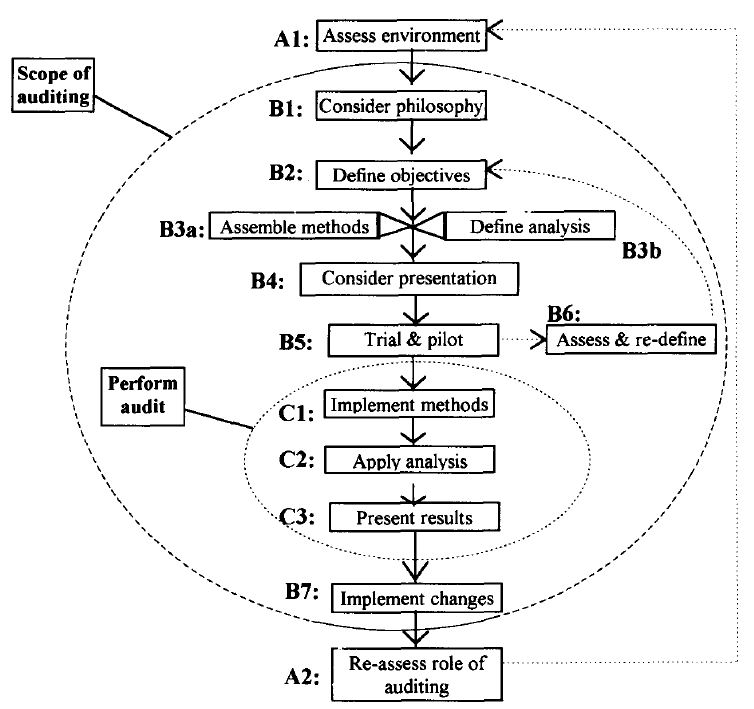
\includegraphics[width=0.5\textwidth]{Overview_of_audit_protocol.JPG}
\centering
\caption{Auditointiprotokolla \cite{dimond} }
\label{auditointi}
\end{figure}

Kuva \ref{auditointi} on jaettu kolmeen osaan, A, B ja C. Tämän protokollan mukaan A ei kuulu auditoinnin piiriin, B on osa auditoinnin strategista kehittämistä, ja C on itse auditoinnin suorittava vaihe \cite{dimond}. Nyt tehty tietosuoja-auditointi vastasi vahvasti kuvan esittämää strategiaa, kuitenkin soveltaen ja hieman kevyemmällä otteella. 

\section{TKO-äly ry:n tietosuoja-auditointi}

Ennen varsinaista auditointia arvioitiin ympäristö, eli mitä auditoidaan ja millä tavoin, kuten kuvassa \ref{auditointi}, \textit{"A1: assessing the environment"}. Kuvan kohdat \textit{"B1: Consideration of philosophy"} sekä \textit{"B2: Definition of objectives"} tehtiin käytännössä yhtenä vaiheena ja yhdessä asiakkaan kanssa, tarkastellen auditoinnin rajoitteita, tavoitteita ja vaatimuksia ennen auditoinnin suorittamista. Kohdat \textit{"B3: Assemble methods \& Define analysis"}, \textit{"B4: Consider presentation"} sekä \textit{"B5: Trial \& pilot"} jäivät auditoinnin suhteen vähemmälle huomiolle. Asiakas oli auditoinnissa hyvin vahvasti mukana ja käytännössä toteutti tekniset muutokset järjestelmiin, näiden osa-alueiden toteutus jäi enemmän asiakkaan kuin auditoijan vastuulle. Näitä kuitenkin käsitellään tässä työssä. Kohdat \textit{"B6: Assess \& redefine"} sekä \textit{"B7: Implement changes"} jakaantuivat sekä asiakkaan että auditoijan välille. Vaikka varsinaisista muutostöistä vastasikin pääasiassa asiakas, niiden asetusten mukaista toimintaa ja toteutusta tarkasteltiin erikseen auditoinnin yhteydessä, sekä sen jälkeen. 

Itse auditointityöhön viittavat kohdat, \textit{"C1: Implement methods"}. \textit{"C2: Apply analysis"} sekä \textit{"C3: Present results"} tehtiin hyvin yhtenäisenä ja manuaalisena toimenpiteenä. Auditointimetodina oli yhdistyksen järjestelmien ja dokumentaation manuaalinen läpikäynti ja tarkastelu tietosuojan näkökulmasta. Tämä tarkoitti käytännössä asiakkaan kanssa yhdessä tietojärjestelmien ja internetsivujen selaamista vaihe vaiheelta, sekä senhetkisten henkilörekisteriselosteiden lukemista. Tämän kartoituksen avulla saimme selville kokonaisvaltaisen kuvan muutosten määrästä, laadusta ja tarpeesta. Varsinaista tulosten esittelyä ei asiakkaalle tai asiakkaan käyttäjille tehty, vaan ne ilmenivät suoraan muuttuvina järjestelyinä yhdistyksen palveluissa.

\subsection{Auditoinnin vaiheet}

Vaikka työ tehtiinkin edellä esitetyn protokollan järjestyksessä, sitä ei tehty minkään sertifikaatin tai standardin pohjalta, vaan enemmänkin tarpeen ja tiedon kautta. Auditointi tehtiin hyvin manuaalisesti asiakkaan kanssa yhteistyössä,  ja tärkein työkalu olikin kommunikaatio asiakkaan edustajien kanssa. Asiakkaan kanssa käytiin läpi heidän käyttämänsä järjestelmät ja dokumentaatio. Jokaisen järjestelmän ja dokumentin läpikäynti oli aikaavievää mutta tarpeellista, kuten tulemme myöhemmin huomaamaan. TKO-äly ry:llä on vahva avoimen datan periaate, joka pyrittiin ottamaan huomioon auditoinnissa ja erityisesti tehtävissä muutoksissa mahdollisuuksien mukaan.

\begin{itemize}
\item - Yhteistyö järjestön webvastaavan kanssa 
\item- Konsultaatioapua Pykälä ry:ltä
\item- HYY:n ja TEK:n lausekkeiden pohjat (LIITTEEKSI?)
\item- Lausekkeiden uudelleenkirjoitus Akin kanssa
\item- Softamuutosten tarkkailu ja uudelleenauditointi (katso vanhat osoitteet läpi, ettei niihen enää pääse)
\end{itemize}

\subsection{Tilanne ennen auditointia}

\begin{itemize}
\item Missä kunnossa asiat oli ennen auditointia
\item dokumentaatio, kuten tietosuojalauseke/rekisteriseloste
\item  datan levittäminen mm googlen palvelimille, eli hallitus käytti Driveä vapaasti datan säilömiseen esim kokouspöytäkirjoja Drivella, kertomatta siitä jäsenistölle
\item  nimien julkaisu websivuilla, eli tapahtumailmoittautumisissa julkaistiin aina kaikkien osallistujien nimet
\item  nimien julkaisu pöytäkirjoissa, eli kaikki tiedot kokoukseen osallistuvista julkaistiin vapaasti internetiit
\item Tärpistö ja tiedostojen nimeäminen, eli tenttien nimet julkaistiin aina tentaattorin nimellä, jolloin näistä muodostui vahingossa henkilörekisteri
\end{itemize}



Tärpistö muutettiin seuraavalla koodilla.

\begin{lstlisting}[language=BASH, inputencoding=utf8, literate= {ä}{{\"a}}1 {ö}{{\"o}}1  {Ä}{{\"A}}1 {Ö}{{\"O}}1 ]
#!/bin/bash

echo "We are here $PWD"

FILES=$PWD/*

for file in $FILES/*
do
  fn="${file##*/}"
  filepath=$(dirname "$file" | sed -e 's/ /_/g; s/-/_/g; s/ä/a/g; s/Ä/A/g; s/Ö/O/g; s/ö/o/g;' | cut -d '/' -f 5)
  mkdir -p $filepath
  mv "$file" $(dirname "$file" | sed -e 's/ /_/g; s/-/_/g; s/ä/a/g; s/Ä/A/g; s/Ö/O/g; s/ö/o/g;' )/${fn:0:7}$filepath${fn: -7}
done
\end{lstlisting}

MITÄ SE TEKEE JA MITEN; MIKSI VIIMEINEN SUBSTITUTION ON HUONO

\begin{lstlisting}[language=BASH,style=tree]
[...]
├── Tietoliikenteen\ perusteet
[...]
│   ├── 140131_Niklander_EK.pdf
│   ├── 140404_Niklander_EK.pdf
│   ├── 140404_Niklander_EK_en.pdf
│   ├── 150410_Niklander_EK.pdf
│   ├── 160129_Karvi_EKpdf.pdf
[...]
│   ├── 171208_Karvi_UK.pdf
│   └── 180126_Niklander_EK.pdf
├── Tietorakenteet
│   ├── 121127_Floreen_EK.pdf
│   ├── 131209_Floreen_KK.pdf
│   ├── 131209_Huttunen_KK.pdf
│   ├── 140128_Floreen_EK.pdf
│   ├── 140224_Floreen_KK1.pdf
│   ├── 140408_Floreen_EK.pdf
│   └── 140408_Floreen_EK_en.pdf
├── Tietorakenteet\ ja\ algoritmit
│   ├── 141024_Laaksonen_KK1.pdf
│   ├── 150302_Floreen_VK1.pdf
│   ├── 150414_Tira_EK.pdf
│   ├── 150506_Floreen_KK2.pdf
│   ├── 150506_Floren_KK2.pdf
[...]
│   ├── 161129_Kivinen_EK.pdf
│   ├── 161220_Verwijnen_KK2.pdf
[...]
\end{lstlisting}

Muuttui muotoon

\begin{lstlisting}[language=BASH,style=tree]
[...]
├── Tietoliikenteen_perusteet
[...]
│   ├── 140131_Tietoliikenteen_perusteet_EK.pdf
│   ├── 140404_Tietoliikenteen_perusteet_EK.pdf
│   ├── 140404_Tietoliikenteen_perusteet_en.pdf
│   ├── 150410_Tietoliikenteen_perusteet_EK.pdf
│   ├── 160129_Tietoliikenteen_perusteetpdf.pdf
[...]
│   ├── 171208_Tietoliikenteen_perusteet_UK.pdf
│   └── 180126_Tietoliikenteen_perusteet_EK.pdf
├── Tietorakenteet
│   ├── 121127_Tietorakenteet_EK.pdf
│   ├── 131209_Tietorakenteet_KK.pdf
│   ├── 140128_Tietorakenteet_EK.pdf
│   ├── 140224_TietorakenteetKK1.pdf
│   ├── 140408_Tietorakenteet_EK.pdf
│   └── 140408_Tietorakenteet_en.pdf
├── Tietorakenteet_ja_algoritmit
│   ├── 141024_Tietorakenteet_ja_algoritmitKK1.pdf
│   ├── 150302_Tietorakenteet_ja_algoritmitVK1.pdf
│   ├── 150414_Tietorakenteet_ja_algoritmit_EK.pdf
│   ├── 150506_Tietorakenteet_ja_algoritmitENG.pdf
│   ├── 150506_Tietorakenteet_ja_algoritmitKK2.pdf
[...]
│   ├── 161129_Tietorakenteet_ja_algoritmit_EK.pdf
│   ├── 161220_Tietorakenteet_ja_algoritmitKK2.pdf
[...]
\end{lstlisting}
	
\begin{itemize}
\item Mitä muutoksia tehtiin
\subitem - uudet lausekkeet
\subitem - nimien ehdollinen julkaisu web-sivuilla
\subitem - nimien julkaisu pöytäkirjoissa (mitä tälle kävi)
\subitem - Tärpistön uudelleennimeäminen, KOODIA YLLÄ
\subitem - Sisäiset prosessit uusittiin (tietojan tallennus Driveen, jos sitä vielä tehdään niin siitä on tiedotettu)
\end{itemize}

\section{Yhteenveto}
Vaikka Suomessa on jo ennen tietosuoja-asetusta hyvin säädelty tietosuojalaki, on sen valvominen ja noudattaminen ollut vailinasta. Uuden asetuksen myötä tullut huomattava sanktio on saanut rekisterinpitäjät huomioimaan tietosuojan paremmin. TÄHÄN JOTAIN TOSI HYVÄÄ KANEETTIA SEKÄ LOPULLISET TULOKSET MITEN KAIKKI TÄMÄ VAIKUTTI TKO-ÄLYN JÄRJESTELMIIN.


% --- References ---
\newpage
\nocite{*}
% one of these or  ...
%\bibliographystyle{plain}
\bibliographystyle{acmfin}
%\bibliographystyle{ieeetr}

% ... or this 
%\bibliographystyle{apalike}

\bibliography{my_references}

\lastpage

\appendices

\pagestyle{empty}

\internalappendix{1}{TKO-Äly ry:n aiempi rekisteriseloste}

\subsection*{1. Rekisterin pitäjä}
TKO-äly ry
PL 68
00014 Helsingin yliopisto

\subsection*{2. Rekisterin nimi}
TKO-äly ry:n jäsenrekisteri

\subsection*{3. Yhteyshenkilö}
Yhdistyksen jäsenvastaava
jasenvastaava@tko-aly.fi

\subsection*{4. Rekisterin käyttötarkoitus}
Jäsenrekisterin tietoja voidaan käyttää yhteydenpitoon jäsenten suuntaan, jäsenmaksujen tarkkailuun ja jäsenyyden tarkastamiseen.

\subsection*{5. Rekisterin tietosisältö}
Täydellinen nimi
Kotikunta
Sähköpostiosoite
Puhelinnumero
Jäsenmaksuun ja jäsenyyteen liittyvät tiedot

\subsection*{6. Rekisterin tietolähteet}
Jäsenhakemuksissa kerätyt tiedot sekä Helsingin yliopiston tietojärjestelmästä saadut tiedot.

\subsection*{7. Tietojen luovutus}
Tietoja voidaan käyttää yhdistyksen toiminnassa yhdistyksen hallituksen ja yhdistyksen sääntöjen määräämällä tavalla.

Yhdistyslain 11 § 2 momentin mukaisesti kaikilla yhdistyksen jäsenillä on oikeus tutustua tietoihin kaikkien jäsenten nimestä, kotipaikasta ja jäsenyydestä.

Tietoja ei luovuteta yhdistyksen ulkopuolelle.

\subsection*{8. Rekisterin suojauksen periaatteet}
Jäsenrekisteri sijaitsee yhdistyksen palvelimella tietokannassa. Palvelin on suojattu ulkopuoliselta käytöltä ja jäsentietojen käyttöä valvotaan. Pääsy rekisteriin on yhdistyksen ATK-järjestelmien ylläpitäjillä sekä jäsenvirkailijoilla. Rekisterinkäyttäjillä on henkilökohtaiset käyttäjätunnukset ja salasanat.

\subsection*{9. Tietojen tarkastusoikeus}
Henkilötietolain 26 § mukaan jäsenellä on oikeus tarkastaa itseään koskevat rekisteritiedot ja saada niistä pyydettäessä kopiot. Tarkastaminen on maksutonta kerran vuodessa.

\pagestyle{empty}

\internalappendix{2}{TKO-Äly ry:n jäsenrekisterin tietosuojaseloste}

\subsection*{Jäsenrekisterin tietosuojaseloste}
Tämä on EU:n yleisen tietosuoja-asetuksen mukainen rekisteri- ja tietosuojaseloste.
Laatimispäivämäärä 21.5.2018. Viimeisin muutos 7.12.2018
\subsection*{1. Rekisterinpitäjä}

TKO-äly ry
PL 68
00014 Helsinki
\subsection*{2. Yhteyshenkilö rekisteriä koskevissa asioissa}

TKO-äly ry:n hallitus
hallitus@tko-aly.fi
\subsection*{3. Rekisterin nimi}

TKO-äly ry:n jäsenrekisteri
\subsection*{4. Oikeusperuste ja henkilötietojen käsittelyn tarkoitus}

EU:n yleisen tietosuoja-asetuksen mukainen oikeusperuste henkilötietojen käsittelylle ovat
rekisterinpitäjän oikeutettu etu ja laillinen velvoite.
Henkilötietojen käsittelyn tarkoitus on yhdistyslain (503/1989) 11§ vaatima jäsenrekisterin
ylläpito, sekä ylläpitää yhdistyksen jäsenten yhteys- ja jäsenyystietoja.

\subsection*{5. Rekisterin tietosisältö}
Täydellinen nimi
Kotikunta
Sähköpostiosoite
Puhelinnumero
Helsingin yliopiston ylioppilaskunnan jäsenyys
Jäsenmaksuun ja jäsenyyteen liittyvät tiedot

\subsection*{6. Säännönmukaiset tietolähteet}
Jäsenhakemuksissa kerätyt yhteystiedot sekä Helsingin yliopiston tietojärjestelmästä tarkistettu opiskelijastatus.

\subsection*{7. Tietojen säännönmukaiset luovutukset}

Soveltuvin osin tietoja voidaan luovuttaa Helsingin Yliopiston Ylioppilaskunnan käyttöön opiskelijakunnan jäsenyyden tarkastamista varten. Muutoin tietoja ei luovuteta kolmansille osapuolille.
\subsection*{8. Tietojen siirto EU:n tai ETA:n ulkopuolelle}

Tietoja voidaan käsitellä Googlen pilvipalveluissa, jolloin käsiteltävät tiedot voivat sijaita EU:n tai ETA:n ulkopuolella. Google on sitoutunut noudattamaan pilvipalvelujensa osalta EU:n yleistä tietosuoja-asetusta ja Privacy Shield viitekehystä.

Edellä mainitun lisäksi tietoja ei siirretä Euroopan unionin tai Euroopan talousalueen ulkopuolelle.

\subsection*{9. Rekisterin suojauksen periaatteet}

Tietojen pääasiallinen säilöntäpaikka on yhdistyksen palvelimella sijaitseva tietokanta. Palvelin on suojattu ulkopuoliselta käytöltä ja jäsentietojen käyttöä valvotaan. Pääsy tietoihin on yhdistyksen tietojärjestelmien pääkäyttäjällä, rajatulla joukolla muita tämän valtuuttamia vastuuhenkilöitä ja yhdistyksen jäsenvastaavalla.

Väliaikaisesti tietoja voidaan käsitellä myös Googlen pilvipalveluissa, jolloin tietoihin on pääsy yhdistyksen jäsenvastaavalla tai laajimmillaan yhdistyksen hallituksella.

Molemmissa edellämainituissa tapauksissa tietojen käsittely edellyttää henkilökohtaista tunnistautumista.

\subsection*{10. Tarkastusoikeus}

Jokaisella rekisteriin kuuluvalla henkilöllä on oikeus tarkistaa rekisteriin hänestä tallennetut tiedot. Tietojen tarkistuspyyntö tulee lähettää kirjallisesti rekisterinpitäjälle. Rekisterinpitäjällä on tarvittaessa oikeus pyytää pyynnön esittäjää todistamaan henkilöllisyytensä. Rekisterinpitäjä vastaa pyynnön esittäjälle EU:n tietosuoja -asetuksessa säädetyssä ajassa (pääsääntöisesti kuukauden kuluessa). Tarkastaminen on maksutonta kerran vuodessa.

\subsection*{11. Oikeus vaatia tiedon korjaamista}

Jokaisella rekisteriin kuuluvalla henkilöllä on oikeus vaatia rekisteriin hänestä talletettujen tietojen korjausta. Tietojen korjauspyyntö tulee lähettää kirjallisesti rekisterinpitäjälle. Rekisterinpitäjällä on tarvittaessa oikeus pyytää pyynnön esittäjää todistamaan henkilöllisyytensä. Rekisterinpitäjä toteuttaa esittäjän pyynnön EU:n tietosuoja-asetuksessa säädetyssä ajassa (pääsääntöisesti kuukauden kuluessa).

\subsection*{12. Muut henkilötietojen käsittelyyn liittyvät tiedot}

Tietoja säilytetään kunnes rekisteröidyn jäsenyys yhdistyksessä päättyy. Jäsenyyden loputtua rekisteröidyn henkilötiedot poistetaan jäsenyyden loppumishetkellä menneillään olevan kalenterivuoden loppuun mennessä.

\subsection*{Poikkeukset:}

Mikäli rekisteröity osallistuu yhdistyksen tai sen hallituksen kokoukseen, kirjataan tämän nimi kokouspöytäkirjaan hyvän pöytäkirjatavan mukaisesti. Yhdistyksiä koskevan kirjanpitovelvoitteen vuoksi kokouspöytäkirjoja säilytetään 10 vuoden ajan.

Yhdistyksen talouden- ja kirjanpitovelvoitteista on määrätty muun muassa kirjanpito- ja yhdistyslaeissa. Täten henkilötiedot, esimerkiksi kirjanpidossa, tositteissa tai muissa vastaavissa talouden ja kirjanpidon asiakirjoissa, säilötään edellä mainittujen lakien mukaisesti vähintään 10 vuoden ajan.



\pagestyle{empty}

\internalappendix{3}{TKO-Äly ry:n tapahtumarekisterin tietosuojaseloste}

\subsection*{Tapahtumarekisterin tietosuojaseloste}
Tämä on EU:n yleisen tietosuoja-asetuksen mukainen rekisteri- ja tietosuojaseloste.
Laatimispäivämäärä 21.5.2018. Viimeisin muutos 24.5.2018

\subsection*{1. Rekisterinpitäjä}
TKO-äly ry
PL 68
00014 Helsinki
\subsection*{2. Yhteyshenkilö rekisteriä koskevissa asioissa}

TKO-äly ry:n hallitus
hallitus@tko-aly.fi

\subsection*{3. Rekisterin nimi}

TKO-äly ry:n tapahtumarekisteri

\subsection*{4. Oikeusperuste ja henkilötietojen käsittelyn tarkoitus}

EU:n yleisen tietosuoja-asetuksen mukainen oikeusperuste henkilötietojen käsittelylle on
rekisterinpitäjän oikeutettu etu.

Henkilötietojen käsittelyn tarkoitus on tapahtumien organisointiin ja niiden maksuliikenteeseen liittyvien toimien mahdollistaminen.

\subsection*{5. Rekisterin tietosisältö}
Koko nimi
Sähköpostiosoite
Puhelinnumero
*Tapahtuman maksutieto
*Erityisruokavalio
*Juomamieltymys
*Mahdolliset tapahtumakohtaiset lisätietokentät
(Tähdellä merkittyjä kenttiä käytetään vain tarvittaessa)

\subsection*{6. Säännönmukaiset tietolähteet}

Tapahtumailmoittautumisen yhteydessä kerätyt tiedot.

\subsection*{7. Tietojen säännönmukaiset luovutukset}

Tapahtumailmoittautumisen yhteydessä ilmoittautujalla on vapaaehtoinen mahdollisuus antaa lupa nimen julkaisuun, jolloin nimi julkaistaan tapahtumaan ilmoittautuneiden listalla.

Edellä mainitun lisäksi tietoja ei julkaista tai luovuteta muille tahoille.

\subsection*{8. Tietojen siirto EU:n tai ETA:n ulkopuolelle}

Tietoja voidaan käsitellä Googlen pilvipalveluissa, jolloin käsiteltävät tiedot voivat sijaita EU:n tai ETA:n ulkopuolella. Google on sitoutunut noudattamaan pilvipalvelujensa osalta EU:n yleistä tietosuoja-asetusta ja Privacy Shield viitekehystä.

Edellä mainitun lisäksi tietoja ei siirretä Euroopan unionin tai Euroopan talousalueen ulkopuolelle.

\subsection*{9. Rekisterin suojauksen periaatteet}

Tietojen pääasiallinen säilöntäpaikka on yhdistyksen palvelimella sijaitseva tietokanta. Palvelin on suojattu ulkopuoliselta käytöltä ja jäsentietojen käyttöä valvotaan. Pääsy tietoihin on yhdistyksen tietojärjestelmien pääkäyttäjällä, rajatulla joukolla muita tämän valtuuttamia vastuuhenkilöitä ja yhdistyksen tapahtumista vastuussa olevilla henkilöillä.

Väliaikaisesti tietoja voidaan käsitellä myös Googlen pilvipalveluissa, jolloin tietoihin on pääsy yhdistyksen jäsenvastaavalla tai laajimmillaan yhdistyksen hallituksella.

Molemmissa edellämainituissa tapauksissa tietojen käsittely edellyttää henkilökohtaista tunnistautumista.

\subsection*{10. Tarkastusoikeus}

Jokaisella rekisteriin kuuluvalla henkilöllä on oikeus tarkistaa rekisteriin hänestä tallennetut tiedot. Tietojen tarkistuspyyntö tulee lähettää kirjallisesti rekisterinpitäjälle. Rekisterinpitäjällä on tarvittaessa oikeus pyytää pyynnön esittäjää todistamaan henkilöllisyytensä. Rekisterinpitäjä vastaa pyynnön esittäjälle EU:n tietosuoja-asetuksessa säädetyssä ajassa (pääsääntöisesti kuukauden kuluessa). Tarkastaminen on maksutonta kerran vuodessa.

\subsection*{11. Oikeus vaatia tiedon korjaamista}

Jokaisella rekisteriin kuuluvalla henkilöllä on oikeus vaatia rekisteriin hänestä talletettujen tietojen korjausta. Tietojen korjauspyyntö tulee lähettää kirjallisesti rekisterinpitäjälle. Rekisterinpitäjällä on tarvittaessa oikeus pyytää pyynnön esittäjää todistamaan henkilöllisyytensä. Rekisterinpitäjä toteuttaa esittäjän pyynnön EU:n tietosuoja-asetuksessa säädetyssä ajassa (pääsääntöisesti kuukauden kuluessa).

\subsection*{12. Muut henkilötietojen käsittelyyn liittyvät tiedot}

Tietoja säilytetään tapahtuman järjestämisajankohdalla menneillään olevan tilikauden tilinpäätöksen vahvistamiseen saakka, kuitenkin enintään kuluvaa kalenterivuotta seuraavan kalenterivuoden huhtikuun loppuun saakka.

\subsection*{Poikkeus:}

Yhdistyksen talouden- ja kirjanpitovelvoitteista on määrätty muun muassa kirjanpito- ja yhdistyslaeissa. Täten henkilötiedot, esimerkiksi kirjanpidossa, tositteissa tai muissa vastaavissa talouden ja kirjanpidon asiakirjoissa, säilötään edellä mainittujen lakien mukaisesti vähintään 10 vuoden ajan.


\pagestyle{empty}

\internalappendix{4}{TKO-Äly ry:n tietosuojapolitiikka}

\subsection*{Tietosuojapolitiikka}
Tämän dokumentin tarkoitus on välittää TKO-äly ry:n tietosuojapolitiikka niille henkilöille, jotka käsittelevät yhdistyksen käytössä olevia henkilörekistereitä. Laatimispäivämäärä 21.5.2018. Viimeisin muutos 27.8.2018

Yhdistyksen käytössä on tällä hetkellä seuraavat rekisterit:

\begin{itemize}
\item Jäsenrekisteri  
\item Tapahtumien ilmoitusrekisteri
\item Kurssikarttasovelluksen käyttäjärekisteri
-\item Fuksipassin käyttäjärekisteri
\end{itemize}
Tämä dokumentti sekä mainittujen rekisterien tietosuojaselosteet tulee päivittää aina kun se on tarpeellista. Edellämainitut tulee tarkistaa ja tarvittaessa päivittää kalenterivuosittain yhdistyksen hallituksen sekä virkailijoiden vaihduttua, viimeistään tammikuun viimeisenä päivänä. Vastuu tietosuojadokumentaation tarkastamisesta ja päivittämisestä on kollektiivisesti yhdistyksen sen hetkisellä hallituksella.

Jokaisen yhdistyksen hallituksen jäsenen ja henkilötietoja käsittelevän virkailijan velvoitetaan tutustuvan ajantasaiseen tietosuojapolitiikkaan ja henkilötietorekistereitä koskeviin tietosuojaselosteisiin.

Yleisesti henkilötietojen käsittelyssä tulee noudattaa pienimmän haitan periaatetta, jonka kohteena on rekisteröity henkilö.


\subsection*{Käyttöoikeudet}

Henkilötietoja sisältävien rekisterien käyttöoikeudet tulee rajata vain niille henkilöille, joille se on välttämätöntä. Käyttöoikeudet tulee päivittää aina kun se on tarpeellista ja tarkistaa kalenterivuosittain, viimeistään tammikuun viimeisenä päivänä. Vastuu käyttöoikeuksien päivittämisestä on yhdistyksen Senior Application Evangelist virkaa hoitavalla vastuuhenkilöllä siltä osin kuin se on mahdollista. Viimekädessä vastuu on kuitenkin kollektiivisesti yhdistyksen senhetkisellä hallituksella.


\subsection*{Henkilötietojen elinkaari}

Henkilötietoja tulee säilyttää vain niin kauan kuin se palvelee alkuperäistä keräystarkoitusta. Tietojen enimmäissäilytysaika tulee määrittää yksityiskohtaisesti jokaisen rekisterin tietosuojaselosteessa.


\subsection*{Tietosuojan tekninen toteutus}

Henkilötietojen suojaamiseen ja säilyvyyteen tulee kiinnittää erityistä huomiota. Käyttöoikeuksien hallinnan ohella käytettyjen ratkaisujen yleinen tietoturva on merkittävässä roolissa. Kaikki tekniset toteutukset tulee toteuttaa parhaan mahdollisen kyseisellä hetkellä vallitsevan tietotaidon ja osaamisen puitteissa. Erityisesti järjestelmien rakentamisessa tulee kiinnittää huomiota EU:n yleisen tietosuoja-asetuksen artiklassa 25 määriteltyyn sisäänrakennetun ja oletusarvoisen tietosuojan periaatteeseen.


\subsection*{Henkilötietojen tarkistus ja korjaus}

Jokaisella rekisteriin kuuluvalla henkilöllä on oikeus tarkistaa rekisteriin hänestä tallennetut tiedot ja pyytää niiden korjausta. Tietojen tarkistus- ja korjauspyynnöt tulee lähettää kirjallisesti rekisterinpitäjälle. Rekisterinpitäjällä on tarvittaessa oikeus pyytää pyynnön esittäjää todistamaan henkilöllisyytensä. Rekisterinpitäjä vastaa rekisteröidyn pyyntöön tai suorittaa rekisteröidyn pyytämän korjauksen EU:n tietosuoja-asetuksessa säädetyssä ajassa (pääsääntöisesti kuukauden kuluessa). Mikäli pyyntöä ei voida toteuttaa kuukauden kuluessa on tästä ilmoitettava rekisteröidylle, jolloin voidaan soveltaa korkeintaan kahden kuukauden lisäaikaa.

Henkilötiedot voi tarkastaa veloituksetta kerran kalenterivuodessa. Myöhemmistä tarkastuspyynnöistä veloitetaan 60€ suuruinen palvelumaksu. Henkilötietojen korjauksesta ei veloiteta koskaan, sillä EU:n yleisen tietosuoja-asetuksen nojalla rekisterinpitäjällä on velvollisuus varmentaa henkilötietojen paikkansapitävyys.


\subsection*{Tietojen julkaisu}

Mikäli halutaan julkaista henkilötietoja, tulee siitä kerätä rekisteröidyltä aina erillinen suostumus ja kyseisen suostumuksen tulee aina olla aidosti vapaaehtoinen. Mahdollisuus henkilötietojen julkaisuun tulee kirjata kyseisen rekisterin tietosuojaselosteeseen. Esimerkiksi tapahtumailmoituksen tapauksessa ilmoittauduttaessa rekisteröidyltä kysytään lupa nimen julkaisemiseen tapahtuman osallistujalistassa. Vaikka lupaa ei annettaisikaan, tapahtumaan voi silti osallistua.

Poikkeuksen edelliseen muodostavat yhdistyksen ja sen hallituksen kokoukset, joihin osallistuvien nimet on kirjattava pöytäkirjaan. Tämän vuoksi kokouskutsuihin tulee kirjata maininta kokoukseen osallistuvien nimen kirjaamisesta kokouksen pöytäkirjaan. Yhdistyksen julkaisemien epävirallisten pöytäkirjojen osalta henkilötiedon julkaisuun tulee kysyä lupa. Julkaisusta kieltäytyneiden nimet voidaan kirjata julkisiin epävirallisiin pöytäkirjoihin anonyyminä tilastotietona.


\end{document}